\documentclass{egee}
\usepackage{comment,alltt}

\def\LB{L\&B}

\title{gLite Job Provenance service User's Guide}
\author{CESNET EGEE JRA1 team}
\DocIdentifier{EGEE-JRA1-??}
\Date{\today}
\Activity{JRA1: Middleware Engineering and Integration}
\DocStatus{DRAFT}
\Dissemination{PUBLIC}
\DocumentLink{}

\Abstract{This user's guide is intended for a user of the Job
  Provenance (JP) service. The service architecture characteristic is
  followed by description of main JP use case scenarios. Technical
  documentation for both JP user and JP administrator is included in
  this document too.  This version of user's guide is part of the
  first release of JP and it also contains release notes describing
  corrent limitations of JP implementation.}

\def\todo#1{\textbf{TODO:} #1}

\begin{document}

%\begin{center}
{\bf Delivery Slip}
\end{center}
\begin{tabularx}{\textwidth}{|l|l|l|X|X|}
\hline
           & {\bf Name} & {\bf Partner} & {\bf Date} & {\bf Signature} \\
\hline
{\bf From} &                  &  & & \\
\hline
{\bf Reviewed by} & &  & & \\

\hline
{\bf Approved by} & & & & \\
\hline
\end{tabularx}

\begin{center}
{\bf Document Change Log}
\end{center}

\begin{tabularx}{\textwidth}{|l|l|X|X|}
\hline
{\bf Issue } & {\bf Date  } & {\bf Comment } & {\bf Author  } \\   \hline

\hline
\end{tabularx}

\begin{center}
{\bf Document Change Record}
\end{center}

\begin{tabularx}{\textwidth}{|l|l|X|}
\hline
{\bf Issue } & {\bf Item  } & {\bf Reason for Change } \\   \hline

\hline
\end{tabularx}

%
% Official text received on October 6, 2004
%
\vfill{\bf Copyright }\copyright{\bf Members of the EGEE Collaboration. 2004. 
See http://eu-egee.org/partners for details on the copyright holders. 

EGEE (``Enabling Grids for E-science in Europe'') is a project funded by
the European Union.  For more information on the project, its partners
and contributors please see http://www.eu-egee.org.

You are permitted to copy and distribute verbatim copies of this
document containing this copyright notice, but modifying this document
is not allowed. You are permitted to copy this document in whole or in
part into other documents if you attach the following reference to the
copied elements: ``Copyright }\copyright{\bf 2004. Members of the EGEE
Collaboration. http://www.eu-egee.org''

The information contained in this document represents the views of
EGEE as of the date they are published. EGEE does not guarantee that
any information contained herein is error-free, or up to date.

EGEE MAKES NO WARRANTIES, EXPRESS, IMPLIED, OR STATUTORY, BY
PUBLISHING THIS DOCUMENT.}


\clearpage

%\newpage
\tableofcontents
\newpage

\section{Job Provenance service overview}
The information about jobs submitted to gLite Workload Management
System is collected by the Logging and Bookkeeping (LB) service.
LB tracks jobs in terms of events and processes them in
a~real time to give overall view on the actual job state. The user may
query the bookkeeping server to obtain either the raw events or the
computed job state, she may also register for receiving notifications
on particular job state changes.

While the LB is intended to keep track of jobs during its lifetime, it
is not supposed to be used for long term archival of such data. The
Job Provenance (JP) service is designed to provide long-term storage
of all data related to job life and allow the end user to perform
data-mining in this data.
The JP is supposed to provide the permanent storage of
the job related information as stored within the \LB, to couple it with
the input sandboxes and other system oriented information necessary to
reproduce the environment where a~particular job run.

\subsection{Gathering data into Job Provenance}
Fig.~\ref{fig:psinter} depicts basic gLite middleware components and
their interaction with the Job Provenance.

\begin{figure}[htpb]
  \centering
  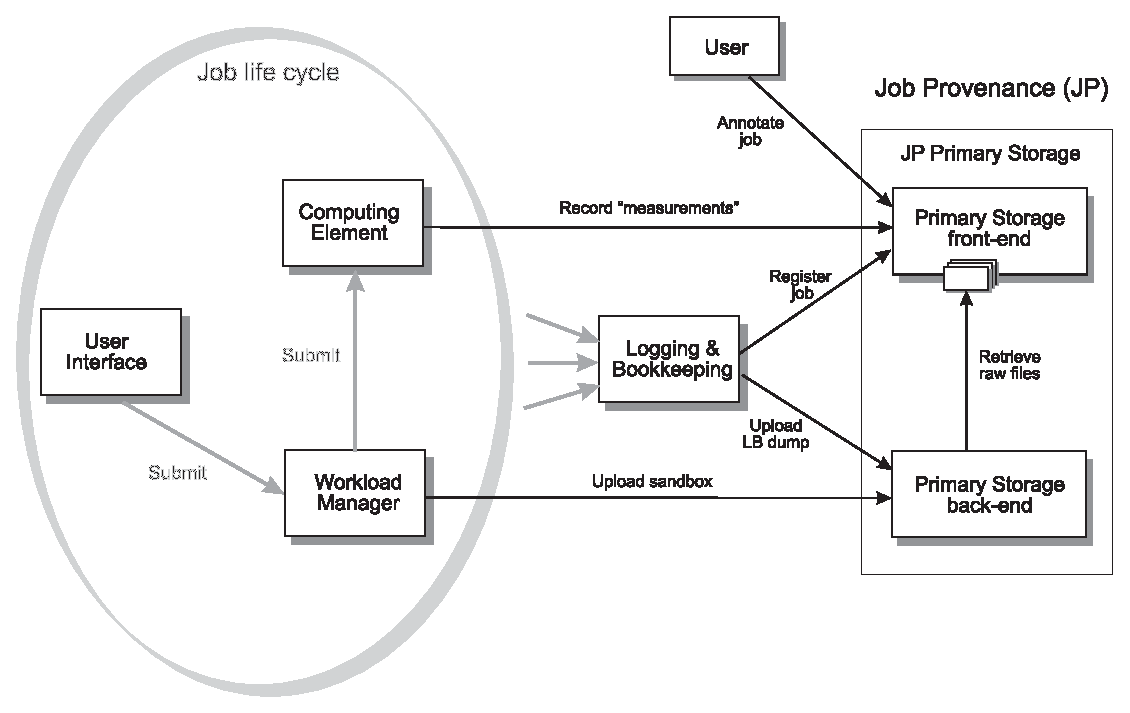
\includegraphics[scale=0.5]{JP-interactions}
  \caption{Data flow into gLite Job Provenance}
  \label{fig:psinter}
\end{figure}

JP is formed of two classes of services: permanent \emph{Primary
Storage} (JPPS) accepts and stores job data while possibly volatile
and configurable \emph{Index Servers} (JPIS) provide an optimized
querying and data-mining interface to the end-users.  The only direct
data retrieval scenario supported by JPPS is the case when user know exact ID
of jobs in the interest.

\subsection{Getting data from Job Provenance}

The role of \emph{Index Servers} (JPIS) is processing and re-arranging the data
from Primary Storage(s) into a~form suitable for frequent and complex user
queries. A user query part of JP is shown in Fig.~\ref{fig:query}.

\begin{figure}[htpb]
  \centering
  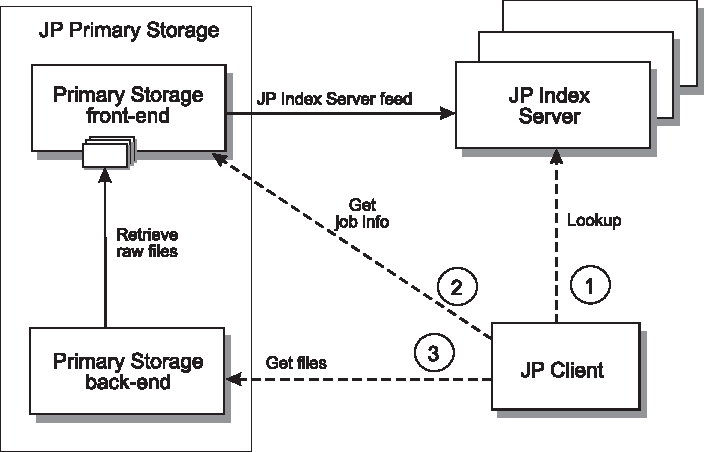
\includegraphics[scale=0.5]{JP-query}
  \caption{Index Server interactions}
  \label{fig:query}
\end{figure}

Index Servers are created, configured, and populated semi-dynamically
according to particular user community needs.  It is responsibility of
its administrator to setup the JPIS with appropriate configuration. There
is no prescribed relationship between Primary Storage and Index Server
installations.  An Index Server may retrieve data from multiple
Primary Storages and vice versa.

The interface exposed by JPIS to the end user is described in the
chapter~\ref{reference}. Command line interface tool for end-user
interface to the JPIS is described in the chapter~\ref{CLI}.


\section{Job Provenance use cases}
\todo{In next release}

\section{Release notes}
\todo{TBD}

\section{Documentation for JP users}

%\subsection{Role of the JP administrator}
% Podle Ljochy sem nepat��. Podle mne mus� u�ivatel v�d�t kdy a s ��m
% otravovat administratora (zejm�na IS).

\subsection{Command line interface (CLI)}
\label{CLI}
{
\newcommand{\dbz}{}
\newcommand{\docbooktolatexpipe}{\ensuremath{|}}
\newskip\docbooktolatexoldparskip
\input glite-jpis-client
}

\subsection{JP web-service interface reference}
\label{reference}

{
\parindent0pt
\def\chapter#1{}
\def\section#1{\subsubsection{#1}}
\def\subsection#1{\par\medskip\textbf{#1}\par}

\let\odesc=\description
\let\oedesc=\enddescription
\renewenvironment{description}{\odesc\itemindent=1em
\listparindent=2em
}{\oedesc}
%\renewenvironment{description}{\list{}{\labelwidth 5cm\leftmargin 5cm}}
%{\endlist}

\let\null=\relax
\input jpws
}



\end{document}
